% Options for packages loaded elsewhere
\PassOptionsToPackage{unicode}{hyperref}
\PassOptionsToPackage{hyphens}{url}
\PassOptionsToPackage{dvipsnames,svgnames,x11names}{xcolor}
\documentclass[
  10pt,
]{article}
\usepackage{xcolor}
\usepackage[margin=0.85in]{geometry}
\usepackage{amsmath,amssymb}
\setcounter{secnumdepth}{5}
\usepackage{iftex}
\ifPDFTeX
  \usepackage[T1]{fontenc}
  \usepackage[utf8]{inputenc}
  \usepackage{textcomp} % provide euro and other symbols
\else % if luatex or xetex
  \usepackage{unicode-math} % this also loads fontspec
  \defaultfontfeatures{Scale=MatchLowercase}
  \defaultfontfeatures[\rmfamily]{Ligatures=TeX,Scale=1}
\fi
\usepackage{lmodern}
\ifPDFTeX\else
  % xetex/luatex font selection
  \setmonofont[]{Menlo}
\fi
% Use upquote if available, for straight quotes in verbatim environments
\IfFileExists{upquote.sty}{\usepackage{upquote}}{}
\IfFileExists{microtype.sty}{% use microtype if available
  \usepackage[]{microtype}
  \UseMicrotypeSet[protrusion]{basicmath} % disable protrusion for tt fonts
}{}
\makeatletter
\@ifundefined{KOMAClassName}{% if non-KOMA class
  \IfFileExists{parskip.sty}{%
    \usepackage{parskip}
  }{% else
    \setlength{\parindent}{0pt}
    \setlength{\parskip}{6pt plus 2pt minus 1pt}}
}{% if KOMA class
  \KOMAoptions{parskip=half}}
\makeatother
\usepackage{color}
\usepackage{fancyvrb}
\newcommand{\VerbBar}{|}
\newcommand{\VERB}{\Verb[commandchars=\\\{\}]}
\DefineVerbatimEnvironment{Highlighting}{Verbatim}{commandchars=\\\{\}}
% Add ',fontsize=\small' for more characters per line
\newenvironment{Shaded}{}{}
\newcommand{\AlertTok}[1]{\textcolor[rgb]{1.00,0.00,0.00}{\textbf{#1}}}
\newcommand{\AnnotationTok}[1]{\textcolor[rgb]{0.38,0.63,0.69}{\textbf{\textit{#1}}}}
\newcommand{\AttributeTok}[1]{\textcolor[rgb]{0.49,0.56,0.16}{#1}}
\newcommand{\BaseNTok}[1]{\textcolor[rgb]{0.25,0.63,0.44}{#1}}
\newcommand{\BuiltInTok}[1]{\textcolor[rgb]{0.00,0.50,0.00}{#1}}
\newcommand{\CharTok}[1]{\textcolor[rgb]{0.25,0.44,0.63}{#1}}
\newcommand{\CommentTok}[1]{\textcolor[rgb]{0.38,0.63,0.69}{\textit{#1}}}
\newcommand{\CommentVarTok}[1]{\textcolor[rgb]{0.38,0.63,0.69}{\textbf{\textit{#1}}}}
\newcommand{\ConstantTok}[1]{\textcolor[rgb]{0.53,0.00,0.00}{#1}}
\newcommand{\ControlFlowTok}[1]{\textcolor[rgb]{0.00,0.44,0.13}{\textbf{#1}}}
\newcommand{\DataTypeTok}[1]{\textcolor[rgb]{0.56,0.13,0.00}{#1}}
\newcommand{\DecValTok}[1]{\textcolor[rgb]{0.25,0.63,0.44}{#1}}
\newcommand{\DocumentationTok}[1]{\textcolor[rgb]{0.73,0.13,0.13}{\textit{#1}}}
\newcommand{\ErrorTok}[1]{\textcolor[rgb]{1.00,0.00,0.00}{\textbf{#1}}}
\newcommand{\ExtensionTok}[1]{#1}
\newcommand{\FloatTok}[1]{\textcolor[rgb]{0.25,0.63,0.44}{#1}}
\newcommand{\FunctionTok}[1]{\textcolor[rgb]{0.02,0.16,0.49}{#1}}
\newcommand{\ImportTok}[1]{\textcolor[rgb]{0.00,0.50,0.00}{\textbf{#1}}}
\newcommand{\InformationTok}[1]{\textcolor[rgb]{0.38,0.63,0.69}{\textbf{\textit{#1}}}}
\newcommand{\KeywordTok}[1]{\textcolor[rgb]{0.00,0.44,0.13}{\textbf{#1}}}
\newcommand{\NormalTok}[1]{#1}
\newcommand{\OperatorTok}[1]{\textcolor[rgb]{0.40,0.40,0.40}{#1}}
\newcommand{\OtherTok}[1]{\textcolor[rgb]{0.00,0.44,0.13}{#1}}
\newcommand{\PreprocessorTok}[1]{\textcolor[rgb]{0.74,0.48,0.00}{#1}}
\newcommand{\RegionMarkerTok}[1]{#1}
\newcommand{\SpecialCharTok}[1]{\textcolor[rgb]{0.25,0.44,0.63}{#1}}
\newcommand{\SpecialStringTok}[1]{\textcolor[rgb]{0.73,0.40,0.53}{#1}}
\newcommand{\StringTok}[1]{\textcolor[rgb]{0.25,0.44,0.63}{#1}}
\newcommand{\VariableTok}[1]{\textcolor[rgb]{0.10,0.09,0.49}{#1}}
\newcommand{\VerbatimStringTok}[1]{\textcolor[rgb]{0.25,0.44,0.63}{#1}}
\newcommand{\WarningTok}[1]{\textcolor[rgb]{0.38,0.63,0.69}{\textbf{\textit{#1}}}}
\usepackage{longtable,booktabs,array}
\newcounter{none} % for unnumbered tables
\usepackage{calc} % for calculating minipage widths
% Correct order of tables after \paragraph or \subparagraph
\usepackage{etoolbox}
\makeatletter
\patchcmd\longtable{\par}{\if@noskipsec\mbox{}\fi\par}{}{}
\makeatother
% Allow footnotes in longtable head/foot
\IfFileExists{footnotehyper.sty}{\usepackage{footnotehyper}}{\usepackage{footnote}}
\makesavenoteenv{longtable}
\usepackage{graphicx}
\makeatletter
\newsavebox\pandoc@box
\newcommand*\pandocbounded[1]{% scales image to fit in text height/width
  \sbox\pandoc@box{#1}%
  \Gscale@div\@tempa{\textheight}{\dimexpr\ht\pandoc@box+\dp\pandoc@box\relax}%
  \Gscale@div\@tempb{\linewidth}{\wd\pandoc@box}%
  \ifdim\@tempb\p@<\@tempa\p@\let\@tempa\@tempb\fi% select the smaller of both
  \ifdim\@tempa\p@<\p@\scalebox{\@tempa}{\usebox\pandoc@box}%
  \else\usebox{\pandoc@box}%
  \fi%
}
% Set default figure placement to htbp
\def\fps@figure{htbp}
\makeatother
\setlength{\emergencystretch}{3em} % prevent overfull lines
\providecommand{\tightlist}{%
  \setlength{\itemsep}{0pt}\setlength{\parskip}{0pt}}
\usepackage{float}\floatplacement{figure}{H}\renewcommand{\thesection}{\alph{section}}
\usepackage{bookmark}
\IfFileExists{xurl.sty}{\usepackage{xurl}}{} % add URL line breaks if available
\urlstyle{same}
\hypersetup{
  pdftitle={CS F429 Natural Language Processing --- Final Report},
  pdfauthor={Name: Roshini Kotte \textbar{} ID Number: 2024A7PS0048H},
  colorlinks=true,
  linkcolor={blue!60!black},
  filecolor={Maroon},
  citecolor={Blue},
  urlcolor={blue!60!black},
  pdfcreator={LaTeX via pandoc}}

\title{\textbf{CS F429 Natural Language Processing --- Final Report}}
\usepackage{etoolbox}
\makeatletter
\providecommand{\subtitle}[1]{% add subtitle to \maketitle
  \apptocmd{\@title}{\par {\large #1 \par}}{}{}
}
\makeatother
\subtitle{Natural Language to SQL: From Rules and LSTMs to Fine-Tuned
Transformers and LLMs}
\author{Name: Roshini Kotte \textbar{} ID Number: 2024A7PS0048H}
\date{}

\begin{document}
\maketitle
\begin{abstract}
We translate English questions into SQLite queries on Spider, a
benchmark whose test databases are never seen in training. Four
generations of methods are compared under one evaluation: a rule-based
template parser and a pointer-generator LSTM (classical), a fine-tuned
T5-base transformer, and gpt-oss-20b, an instruction-tuned large
language model used without training. Our contribution is a two-part
decoding method for T5 that targets its main error, naming tables and
columns that do not exist: (A) schema-constrained beam search, which
discards candidates that use unknown identifiers and checks finished
candidates with SQLite, and (B) execution-guided reranking, which keeps
the first candidate that runs. On Spider dev, A + B raises T5-base from
54.1\% to 64.4\% execution accuracy (+10.3 points, 95\% CI {[}7.5,
13.3{]}) and cuts invalid SQL from 31\% to 13\%, without retraining. On
the held-out Spider test set (2,147 questions, run once) it raises
T5-base from 53.4\% to 62.4\% (+9.0 points, 95\% CI {[}7.3, 10.9{]}),
fixing 196 questions and breaking 3. gpt-oss-20b reaches 78.6\%
execution accuracy zero-shot but only 20.1\% exact match, which shows
that exact match penalises correct SQL written in a different style.
\end{abstract}

\section{Introduction to the NLP
Task}\label{introduction-to-the-nlp-task}

\subsection{Motivation}\label{motivation}

Most structured data in companies, hospitals and universities lives in
relational databases. Querying them requires knowing SQL and the exact
table and column names of each database. Text-to-SQL removes this
barrier: given the question \emph{``How many singers are from France?''}
and a database, the system writes
\texttt{SELECT\ count(*)\ FROM\ singer\ WHERE\ country\ =\ \textquotesingle{}France\textquotesingle{}},
runs it and returns the answer. Non-programmers can then ask questions
of their data directly.

\subsection{Core challenges}\label{core-challenges}

\begin{enumerate}
\def\labelenumi{\arabic{enumi}.}
\tightlist
\item
  \textbf{Schema linking.} Question words must be matched to the right
  tables and columns, which rarely share the same spelling (``singers''
  → table \texttt{singer}, ``older than 30'' → column \texttt{Age}).
\item
  \textbf{Structure.} Many questions need joins across tables, grouping,
  ordering, nested queries or set operations.
\item
  \textbf{Unseen databases.} Spider's test databases never appear in
  training, so a model must read the schema it is given rather than
  memorise names.
\item
  \textbf{Executability.} A single wrong column name makes SQLite reject
  the whole query, so an almost-correct query still scores zero.
\end{enumerate}

\subsection{Formulation}\label{formulation}

Given a question \(Q\) and a database schema \(S\) (tables, columns and
foreign keys), produce the SQL query \(Y\) that answers \(Q\). All our
neural models generate \(Y\) one token at a time, choosing at each step
a likely next token given the question, the schema and the tokens
written so far:
\[\hat{Y}=\arg\max_Y \prod_{t=1}^{n} P(y_t\mid y_{<t},Q,S).\]

\section{Literature Survey: Why the Problem
Matters}\label{literature-survey-why-the-problem-matters}

\textbf{Rule-based systems.} PRECISE (Popescu et al., 2003) maps
question words to database elements with hand-written rules and is very
precise on questions it accepts, but fails on anything outside its
patterns. Grammar-based parsers (Zettlemoyer and Collins, 2005; Wong and
Mooney, 2007) need a hand-built lexicon for every new domain.

\textbf{Neural sequence-to-sequence models.} LSTM encoder--decoders
(Hochreiter and Schmidhuber, 1997; Sutskever et al., 2014) with
attention (Bahdanau et al., 2015) treat Text-to-SQL as translation.
Pointer networks (Vinyals et al., 2015; See et al., 2017) let the
decoder copy table names and values from the input. On WikiSQL, Seq2SQL
(Zhong et al., 2017) and SQLNet (Xu et al., 2017) fill SQL sketches. On
Spider these models reach only 4--12\% exact match (Yu et al., 2018),
mostly because they cannot link question words to unseen schemas. Our
Part 2 baselines belong here.

\textbf{Pre-trained transformers.} The transformer (Vaswani et al.,
2017) replaces recurrence with self-attention. T5 (Raffel et al., 2020)
is a transformer encoder--decoder pre-trained on a large web corpus;
fine-tuned on Spider with the schema written into the input, it became a
strong and simple baseline (Shaw et al., 2021). Relation-aware encoders
such as RAT-SQL (Wang et al., 2020) model links between question words
and schema items. PICARD (Scholak et al., 2021) showed that
\emph{constraining decoding}, rejecting invalid partial SQL during beam
search, adds several points to T5, and RESDSQL (Li et al., 2023) ranks
schema items before decoding. Our novelty follows PICARD's idea in a
lighter form.

\textbf{Large language models (LLMs).} Instruction-tuned LLMs write SQL
from a prompt with no task-specific training. DIN-SQL (Pourreza and
Rafiei, 2023) and DAIL-SQL (Gao et al., 2024) prompt GPT-4 with the
schema written as \texttt{CREATE\ TABLE} statements and a few solved
examples, reaching about 85\% execution accuracy on Spider. Feeding
execution errors back to the model (``self-debugging''; Chen et al.,
2024) is a common addition. We use the open-weight gpt-oss-20b (OpenAI,
2025) since hosted APIs were not available to us.

\textbf{Why it matters.} Natural-language access to databases is one of
the most practical applications of NLP, and Spider's unseen-database
split tests exactly the generalisation that real users need.

\section{Dataset}\label{dataset}

\subsection{Datasets and splits}\label{datasets-and-splits}

{\def\LTcaptype{none} % do not increment counter
\begin{longtable}[]{@{}
  >{\raggedright\arraybackslash}p{(\linewidth - 4\tabcolsep) * \real{0.3333}}
  >{\raggedright\arraybackslash}p{(\linewidth - 4\tabcolsep) * \real{0.3333}}
  >{\raggedright\arraybackslash}p{(\linewidth - 4\tabcolsep) * \real{0.3333}}@{}}
\toprule\noalign{}
\begin{minipage}[b]{\linewidth}\raggedright
\end{minipage} & \begin{minipage}[b]{\linewidth}\raggedright
Spider (Yu et al., 2018)
\end{minipage} & \begin{minipage}[b]{\linewidth}\raggedright
WikiSQL (Zhong et al., 2017)
\end{minipage} \\
\midrule\noalign{}
\endhead
\bottomrule\noalign{}
\endlastfoot
Domain & 138 domains (college, business, sport, entertainment, \ldots) &
Wikipedia tables (open domain) \\
Source and licence & \texttt{yale-lily.github.io/spider} (CC BY-SA 4.0)
& \texttt{github.com/salesforce/WikiSQL} (BSD-3) \\
Size & 7,000 train / 1,034 dev / 2,147 test questions & 56,355 train /
8,421 dev / 15,878 test \\
Databases & 140 / 20 / 40, no overlap between splits (verified) & One
table per question \\
SQL operations & Joins, \texttt{GROUP\ BY}, \texttt{HAVING},
\texttt{ORDER\ BY}, nesting, set operations & \texttt{SELECT}, one
aggregate, \texttt{AND} conditions \\
Role here & Main benchmark, all models & Part 2 LSTM warm-up and
single-table sanity check \\
\end{longtable}
}

\textbf{Why these datasets.} Spider is the standard benchmark for
multi-table Text-to-SQL on unseen databases, and every question ships
with an executable SQLite database, so predictions can be checked by
running them. WikiSQL is large and simple, which made it a useful
warm-up for the LSTM.

\textbf{Spider statistics.} Spider labels each question by difficulty.
Dev has 248 easy, 446 medium, 174 hard and 166 extra-hard questions;
test has 470 / 857 / 463 / 357. By structure, dev has 544 single-table,
438 multi-table (join or set operation) and 52 nested questions; test
has 1,100 / 908 / 139. All 7,000 / 1,034 / 2,147 Spider questions load
without exclusions.

\subsection{Preprocessing}\label{preprocessing}

\textbf{Schema serialisation for T5.} The question and the database
schema are joined into one line: the question, the database name, then
each table with its columns, then the foreign keys. This is the real
input for dev question 4 (198 tokens):

\begin{Shaded}
\begin{Highlighting}[]
\NormalTok{What is the average, minimum, and maximum age of all singers from France? | concert\_singer}
\NormalTok{| concert : Stadium\_ID , Theme , Year , concert\_ID , concert\_Name}
\NormalTok{| singer : Age , Country , Is\_male , Name , Singer\_ID , Song\_Name , Song\_release\_year}
\NormalTok{| singer\_in\_concert : Singer\_ID , concert\_ID | stadium : ... | fk : concert.Stadium\_ID {-}\textgreater{} stadium.Stadium\_ID ...}
\end{Highlighting}
\end{Shaded}

\textbf{Tokenisation.} T5 uses a SentencePiece sub-word vocabulary
(32,000 pieces), so a rare name is split into known pieces instead of
becoming an unknown word: \texttt{singers} → \texttt{▁singer}
\texttt{s}, \texttt{concert\_singer} → \texttt{▁concert} \texttt{\_}
\texttt{s} \texttt{inger}. No lower-casing, stemming or stop-word
removal is applied, because table names, values and SQL keywords must be
reproduced exactly.

\textbf{Fixing the vocabulary.} T5's vocabulary has no
\texttt{\textless{}} character. With the original tokenizer,
\texttt{WHERE\ age\ \textless{}\ 30} becomes
\texttt{...\ ▁age\ ▁\ \textless{}unk\textgreater{}\ ▁30}, so the model
could never write ``less than''. This affected \textbf{320 of 7,000
training} and \textbf{42 of 1,034 dev} gold queries. We added
\texttt{\textless{}} and \texttt{\textless{}=} as new tokens (and
enlarged T5's embedding table to match) before fine-tuning; afterwards
no gold query contains an unknown token and the same SQL becomes
\texttt{...\ ▁age\ \textless{}\ ▁30}.

{\def\LTcaptype{none} % do not increment counter
\begin{longtable}[]{@{}
  >{\raggedright\arraybackslash}p{(\linewidth - 8\tabcolsep) * \real{0.1579}}
  >{\raggedleft\arraybackslash}p{(\linewidth - 8\tabcolsep) * \real{0.2105}}
  >{\raggedleft\arraybackslash}p{(\linewidth - 8\tabcolsep) * \real{0.2105}}
  >{\raggedleft\arraybackslash}p{(\linewidth - 8\tabcolsep) * \real{0.2105}}
  >{\raggedleft\arraybackslash}p{(\linewidth - 8\tabcolsep) * \real{0.2105}}@{}}
\toprule\noalign{}
\begin{minipage}[b]{\linewidth}\raggedright
Spider split
\end{minipage} & \begin{minipage}[b]{\linewidth}\raggedleft
Questions
\end{minipage} & \begin{minipage}[b]{\linewidth}\raggedleft
Input tokens (mean / max)
\end{minipage} & \begin{minipage}[b]{\linewidth}\raggedleft
Inputs over 512 tokens
\end{minipage} & \begin{minipage}[b]{\linewidth}\raggedleft
SQL tokens (mean / max)
\end{minipage} \\
\midrule\noalign{}
\endhead
\bottomrule\noalign{}
\endlastfoot
Train & 7,000 & 352 / 2,255 & 1,669 (24\%) & 44 / 245 \\
Dev & 1,034 & 246 / 776 & 78 (8\%) & 42 / 160 \\
Test & 2,147 & 251 / 872 & 196 (9\%) & 45 / 249 \\
\end{longtable}
}

Inputs longer than 512 tokens are truncated, which cuts off the last
tables of very large schemas (a limitation discussed in §e).

\textbf{Prompt format for the LLM.} gpt-oss-20b instead receives the
schema as SQL \texttt{CREATE\ TABLE} statements with primary and foreign
keys and three example rows per table, following DAIL-SQL (Gao et al.,
2024):

\begin{Shaded}
\begin{Highlighting}[]
\NormalTok{CREATE TABLE "singer" ( "Singer\_ID" INTEGER, "Name" TEXT, "Country" TEXT, "Age" INTEGER, ...}
\NormalTok{  PRIMARY KEY ("Singer\_ID") );}
\NormalTok{/* 3 example rows: Singer\_ID | Name | Country | Age ...  1 | Joe Sharp | Netherlands | 52 ... */}
\NormalTok{Question: What is the average, minimum, and maximum age of all singers from France?}
\end{Highlighting}
\end{Shaded}

\subsection{Dataset limitations}\label{dataset-limitations}

Spider is English-only and skewed towards college, business and
entertainment schemas. Dev has only 20 databases, so results vary
strongly by database. Most queries appear with two paraphrased
questions. Small databases allow a wrong query to return the right
answer by coincidence (an example appears in §e). Gold SQL follows
inconsistent conventions (quoting, capitalisation, trailing semicolons),
and one training query refers to a table missing from its database.
Difficulty is imbalanced: 43\% of dev is medium and 16\% extra-hard.

\section{Method}\label{method}

\subsection{Classical baselines (Part
2)}\label{classical-baselines-part-2}

\textbf{Template parser.} Hand-written rules match question words to the
table and columns of one table, detect values (numbers, quoted names),
comparison phrases (``older than'' → \texttt{\textgreater{}}),
aggregation cues (``how many'' → \texttt{COUNT}, ``average'' →
\texttt{AVG}) and ordering cues, and fill a single-table
\texttt{SELECT\ ...\ FROM\ ...\ WHERE\ ...\ ORDER\ BY} template. It
never joins tables, and returns nothing when it cannot match a question
confidently (8.9\% of dev questions).

\textbf{Pointer-generator LSTM.}

{\def\LTcaptype{none} % do not increment counter
\begin{longtable}[]{@{}
  >{\raggedright\arraybackslash}p{(\linewidth - 2\tabcolsep) * \real{0.5000}}
  >{\raggedright\arraybackslash}p{(\linewidth - 2\tabcolsep) * \real{0.5000}}@{}}
\toprule\noalign{}
\begin{minipage}[b]{\linewidth}\raggedright
Component
\end{minipage} & \begin{minipage}[b]{\linewidth}\raggedright
Setting
\end{minipage} \\
\midrule\noalign{}
\endhead
\bottomrule\noalign{}
\endlastfoot
Encoder & 2-layer bidirectional LSTM, embedding 256, hidden 256 per
direction \\
Decoder & 2-layer LSTM, hidden 512, additive attention over the encoder
states \\
Copy mechanism & A learned gate mixes ``generate a word from the
vocabulary'' with ``copy a word from the input'' \\
Vocabulary & 102,463 word types from training data; word-level
embeddings \\
Training & Adam, learning rate 1e-3, batch 64, dropout 0.2; WikiSQL 10
epochs, then Spider 25 epochs \\
Decoding & Greedy, at most 128 tokens, then rendering and schema-aware
repair \\
\end{longtable}
}

\emph{How its weights were learned.} Every weight, including the word
embeddings, started as a small random number. For each training example
the model predicted the gold SQL one token at a time; the loss was how
improbable it found the correct token (cross-entropy). Backpropagation
computed how each weight should change to reduce that loss, and the Adam
optimiser applied the change. Repeating this over all examples for
several epochs gives the trained weights. Nothing was pre-trained or
frozen.

\subsection{Modern model 1: fine-tuned
T5-base}\label{modern-model-1-fine-tuned-t5-base}

\textbf{Architecture.} T5-base (Raffel et al., 2020) is a transformer
encoder--decoder with 220 million parameters. The encoder (12 layers)
reads the whole input; the decoder (12 layers) writes the SQL token by
token. Each layer uses \textbf{self-attention}: every token computes a
weighted average over all other tokens, with weights based on how
relevant they are, so the word ``singers'' can directly attend to the
column \texttt{singer} anywhere in the schema. This replaces the LSTM's
step-by-step recurrence, which had to carry information through every
position. The decoder also attends to the encoder's output, like the
LSTM's attention. Each layer has 12 attention heads and a feed-forward
block; the model dimension is 768. Positions are encoded as relative
distances.

\textbf{How its weights are learned.} Unlike the LSTM, T5 does not start
from random weights. Google pre-trained it on a large English web corpus
(C4) by hiding random spans of text and training it to fill them in, so
it already understands English and some code. We start from that
checkpoint and \textbf{fine-tune}: we show it (question + schema → gold
SQL) pairs and update \textbf{all} its weights by backpropagation to
make the gold SQL more probable, using the same cross-entropy loss as
the LSTM. Only the embeddings of the two new tokens
(\texttt{\textless{}}, \texttt{\textless{}=}) start from scratch.
Because fine-tuning adjusts knowledge the model already has, T5 learns
far more from Spider's 7,000 examples than the LSTM could.

\textbf{Why T5.} It is the standard pre-trained baseline for Spider,
takes the schema as plain text, needs no task-specific architecture, and
fits in half a GPU for training.

{\def\LTcaptype{none} % do not increment counter
\begin{longtable}[]{@{}
  >{\raggedright\arraybackslash}p{(\linewidth - 2\tabcolsep) * \real{0.5000}}
  >{\raggedright\arraybackslash}p{(\linewidth - 2\tabcolsep) * \real{0.5000}}@{}}
\toprule\noalign{}
\begin{minipage}[b]{\linewidth}\raggedright
Setting
\end{minipage} & \begin{minipage}[b]{\linewidth}\raggedright
Value
\end{minipage} \\
\midrule\noalign{}
\endhead
\bottomrule\noalign{}
\endlastfoot
Checkpoint & \texttt{google-t5/t5-base} (220M parameters, all trainable,
none frozen) \\
Training data & Spider train, 7,000 questions \\
Max input / output length & 512 / 256 tokens \\
Optimiser & AdamW, learning rate 3e-4, linear decay with 5\% warm-up,
gradient clipping 1.0 \\
Batch size, epochs, seed & 16, 25 epochs (about 36 minutes), seed 42 \\
Checkpoint selection & Epoch with the best dev execution accuracy,
measured after every epoch (epoch 14) \\
Decoding & Beam search with 4 or 8 beams \\
\end{longtable}
}

\subsection{Modern model 2: gpt-oss-20b (instruction-tuned
LLM)}\label{modern-model-2-gpt-oss-20b-instruction-tuned-llm}

gpt-oss-20b (OpenAI, 2025) is an open-weight transformer
\textbf{decoder} (24 layers, 21 billion parameters). It is a
mixture-of-experts model: each layer has 32 expert feed-forward blocks
and uses only 4 per token, so about 3.6 billion parameters are active
for each token. It was pre-trained on large text and code corpora and
then trained to follow instructions and reason before answering.
\textbf{We do not train it}: all its weights stay frozen and the task is
given entirely in the prompt (in-context learning).

{\def\LTcaptype{none} % do not increment counter
\begin{longtable}[]{@{}
  >{\raggedright\arraybackslash}p{(\linewidth - 2\tabcolsep) * \real{0.5000}}
  >{\raggedright\arraybackslash}p{(\linewidth - 2\tabcolsep) * \real{0.5000}}@{}}
\toprule\noalign{}
\begin{minipage}[b]{\linewidth}\raggedright
Setting
\end{minipage} & \begin{minipage}[b]{\linewidth}\raggedright
Value
\end{minipage} \\
\midrule\noalign{}
\endhead
\bottomrule\noalign{}
\endlastfoot
Prompt & Instruction + schema as \texttt{CREATE\ TABLE} with keys + 3
sample rows per table + question \\
Few-shot examples & 0 or 3, the most similar Spider train questions
(word-overlap cosine), always from other databases \\
Decoding & Greedy, at most 1,024 new tokens, reasoning effort ``low'';
SQL extracted from the reply \\
Error feedback (B) & Up to 2 retries with the SQLite error message \\
Precision & bfloat16 (about 42 GB); the faster 4-bit kernels could not
be compiled on the HPC \\
\end{longtable}
}

\textbf{Why gpt-oss-20b.} It represents the current generation
(instruction-tuned LLMs, as allowed by the course brief), its weights
are public so results are reproducible, and it fits on our HPC GPU.

\subsection{Our contribution: schema-constrained decoding (A) and
execution-guided reranking
(B)}\label{our-contribution-schema-constrained-decoding-a-and-execution-guided-reranking-b}

\textbf{Motivation.} With T5 as with the LSTM, the main error is
\textbf{schema linking}: on Spider dev, 317 of T5's 1,034 queries (31\%)
do not run, and 275 of those fail with ``no such column''. Beam search
already produces several candidate queries per question, and a
lower-ranked candidate is often correct. A and B choose a better
candidate. Neither needs retraining; both work on the trained T5.

\textbf{A: schema-constrained beam search.} Beam search keeps the
\emph{k} most probable partial queries at each step.

\begin{enumerate}
\def\labelenumi{\arabic{enumi}.}
\tightlist
\item
  Before decoding, build the set of allowed words: SQL keywords, every
  table and column name of \emph{this} database, table aliases
  (\texttt{T1}, \texttt{T2}, \ldots), aliases the query itself declares
  (\texttt{AS\ total}), numbers, and the words of the question (for
  unquoted values).
\item
  At every decoding step, look at each beam's last \emph{completed}
  word. If it is not allowed, discard the beam (set all its next-token
  scores to minus infinity). A word still being written is not judged,
  and text inside quotes (values) is never checked.
\item
  When decoding ends, check each finished candidate with SQLite
  \texttt{EXPLAIN}, which compiles the query without running it and
  fails on unknown tables or columns and on syntax errors. Return the
  first candidate that compiles, or the top beam if none does.
\end{enumerate}

\textbf{B: execution-guided reranking.} Run the \emph{k} candidates in
order on the database (read-only, 5-second limit each). Return the first
that runs and returns rows; if none returns rows, the first that runs;
if none runs, the top beam. An empty result is treated only as weaker
evidence than a non-empty one, never as proof of correctness. For the
LLM, which produces one answer rather than a beam, B instead sends the
SQLite error back to the model and asks for a corrected query, at most
twice.

\textbf{A + B} applies B to the candidates that survive A.

\emph{Example (concert\_singer).} For ``List singer names and number of
concerts for each singer'', plain T5 writes
\texttt{...\ FROM\ concert\ AS\ T1\ JOIN\ singer\ AS\ T2\ ON\ T1.singer\_id\ =\ T2.singer\_id\ ...},
which fails because \texttt{concert} has no \texttt{singer\_id}. With A
+ B the chosen candidate joins \texttt{singer\_in\_concert} and is
correct.

\textbf{What is new.} PICARD constrains T5 with a full incremental SQL
parser. Ours needs no parser: it checks completed words against the
schema, then relies on SQLite itself (\texttt{EXPLAIN}, then execution)
to judge whole queries. It is simple, works with any seq2seq model and
any SQLite database, and directly targets the schema-linking errors
found in our error analysis.

{\def\LTcaptype{none} % do not increment counter
\begin{longtable}[]{@{}ll@{}}
\toprule\noalign{}
Hyperparameter & Value \\
\midrule\noalign{}
\endhead
\bottomrule\noalign{}
\endlastfoot
Beams \emph{k} (candidates kept) & 8 \\
Constraint check & Every decoding step, completed bare words only \\
Final check & SQLite \texttt{EXPLAIN} on finished candidates \\
Rerank & First candidate that executes with rows, 5-second limit \\
LLM correction retries & 2 \\
\end{longtable}
}

\emph{Check that A never blocks correct SQL.} Applied to the gold
queries themselves, the constraint rejects 0 of 1,034 dev and 1 of 7,000
train queries; that one names a table missing from its database (a
Spider annotation error).

\subsection{Implementation}\label{implementation}

Python 3.12, PyTorch 2.14, Hugging Face Transformers 5.20, SQLite
(read-only connections) and the official Spider evaluator; training and
decoding ran as Slurm jobs on the BITS HPC, and evaluation and the demo
run on a laptop. The environment is pinned with \texttt{uv}; 106 unit
tests cover data loading, the models, the constraint, the reranker and
the metrics.

\section{Experiments}\label{experiments}

\subsection{Set up}\label{set-up}

All systems answer the same questions and are scored by the same
evaluator. Every choice (checkpoint, beam size, prompts) was made on
Spider dev. The Spider test set (2,147 questions, 40 databases never
used for any decision) was run \textbf{once}, at the end. Each LLM
setting and the T5 ablation was run as a separate HPC job.

\subsection{Metrics}\label{metrics}

\begin{itemize}
\tightlist
\item
  \textbf{Execution accuracy (EX).} Run the predicted and gold SQL on
  the database and compare the results (as a multiset of rows; order
  matters only if the gold query has \texttt{ORDER\ BY}). This is the
  most meaningful metric: it rewards any query that gets the right
  answer, however it is written. \emph{Limitation:} a wrong query can
  return the right rows by coincidence on a small database.
\item
  \textbf{Exact-set match (EM).} Compare each clause of the predicted
  and gold query (\texttt{SELECT}, \texttt{WHERE}, \texttt{GROUP\ BY},
  \ldots) as sets, ignoring values. \emph{Limitation:} a correct query
  written differently (an alias, a \texttt{LEFT\ JOIN}, a subquery
  instead of a join) counts as wrong.
\item
  \textbf{Invalid-SQL rate.} Share of predictions that fail to run,
  split by SQLite error type. It shows directly whether the model
  respects the schema.
\end{itemize}

BLEU-style text-overlap metrics are not used: two queries can share most
tokens yet return different answers. EX and EM come from the official
Spider evaluator. For significance we report a 95\% confidence interval
that resamples whole databases (questions on the same database are
correlated) and McNemar's test on paired per-question outcomes.

\subsection{Baselines}\label{baselines}

Classical: template parser and pointer-generator LSTM. Modern: T5-base
with beam search; gpt-oss-20b zero-shot and few-shot. Ours: T5-base + A,
+ B and + A + B, and gpt-oss-20b + B (error feedback).

\subsection{Evaluation, Results and
Discussion}\label{evaluation-results-and-discussion}

\textbf{Main results (official evaluator).}

{\def\LTcaptype{none} % do not increment counter
\begin{longtable}[]{@{}
  >{\raggedright\arraybackslash}p{(\linewidth - 10\tabcolsep) * \real{0.3333}}
  >{\raggedright\arraybackslash}p{(\linewidth - 10\tabcolsep) * \real{0.2667}}
  >{\raggedleft\arraybackslash}p{(\linewidth - 10\tabcolsep) * \real{0.1000}}
  >{\raggedleft\arraybackslash}p{(\linewidth - 10\tabcolsep) * \real{0.1000}}
  >{\raggedleft\arraybackslash}p{(\linewidth - 10\tabcolsep) * \real{0.1000}}
  >{\raggedleft\arraybackslash}p{(\linewidth - 10\tabcolsep) * \real{0.1000}}@{}}
\toprule\noalign{}
\begin{minipage}[b]{\linewidth}\raggedright
System
\end{minipage} & \begin{minipage}[b]{\linewidth}\raggedright
Type
\end{minipage} & \begin{minipage}[b]{\linewidth}\raggedleft
Dev EX
\end{minipage} & \begin{minipage}[b]{\linewidth}\raggedleft
Dev EM
\end{minipage} & \begin{minipage}[b]{\linewidth}\raggedleft
Test EX
\end{minipage} & \begin{minipage}[b]{\linewidth}\raggedleft
Test EM
\end{minipage} \\
\midrule\noalign{}
\endhead
\bottomrule\noalign{}
\endlastfoot
Template parser & Rules & 9.9\% & 5.9\% & 9.5\% & 6.7\% \\
Pointer-generator LSTM & Classical neural & 8.1\% & 5.0\% & 7.2\% &
5.5\% \\
T5-base, beam & Fine-tuned transformer & 54.1\% & 52.1\% & 53.4\% &
49.6\% \\
\textbf{T5-base + A + B (ours)} & Fine-tuned + novelty & \textbf{64.4\%}
& \textbf{59.5\%} & \textbf{62.4\%} & \textbf{56.7\%} \\
gpt-oss-20b, 0-shot & LLM, no training & 78.6\% & 20.1\% & --- & --- \\
gpt-oss-20b, 0-shot + B & LLM + error feedback & 78.7\% & 20.1\% & --- &
--- \\
gpt-oss-20b, 3-shot & LLM, no training & 81.2\% & 32.5\% & {[}TEST{]} &
{[}TEST{]} \\
\end{longtable}
}

The table shows how the field has moved. Rules and LSTMs answer fewer
than one question in ten; fine-tuning a pre-trained transformer answers
over half; our decoding raises that to about two thirds; an
instruction-tuned LLM answers about four in five with no task-specific
training.

\textbf{Ablation of A and B (T5-base, 8 beams, official evaluator).}

{\def\LTcaptype{none} % do not increment counter
\begin{longtable}[]{@{}
  >{\raggedright\arraybackslash}p{(\linewidth - 12\tabcolsep) * \real{0.1111}}
  >{\raggedleft\arraybackslash}p{(\linewidth - 12\tabcolsep) * \real{0.1481}}
  >{\raggedleft\arraybackslash}p{(\linewidth - 12\tabcolsep) * \real{0.1481}}
  >{\raggedleft\arraybackslash}p{(\linewidth - 12\tabcolsep) * \real{0.1481}}
  >{\raggedleft\arraybackslash}p{(\linewidth - 12\tabcolsep) * \real{0.1481}}
  >{\raggedleft\arraybackslash}p{(\linewidth - 12\tabcolsep) * \real{0.1481}}
  >{\raggedleft\arraybackslash}p{(\linewidth - 12\tabcolsep) * \real{0.1481}}@{}}
\toprule\noalign{}
\begin{minipage}[b]{\linewidth}\raggedright
Decoding
\end{minipage} & \begin{minipage}[b]{\linewidth}\raggedleft
Dev EX
\end{minipage} & \begin{minipage}[b]{\linewidth}\raggedleft
Dev EM
\end{minipage} & \begin{minipage}[b]{\linewidth}\raggedleft
Dev invalid
\end{minipage} & \begin{minipage}[b]{\linewidth}\raggedleft
Test EX
\end{minipage} & \begin{minipage}[b]{\linewidth}\raggedleft
Test EM
\end{minipage} & \begin{minipage}[b]{\linewidth}\raggedleft
Test invalid
\end{minipage} \\
\midrule\noalign{}
\endhead
\bottomrule\noalign{}
\endlastfoot
Beam search (baseline) & 54.1\% & 52.1\% & 30.7\% & 53.4\% & 49.6\% &
30.8\% \\
+ A, pruning only & 55.1\% & 52.9\% & 28.2\% & 55.4\% & 51.2\% &
27.6\% \\
+ A, pruning + \texttt{EXPLAIN} check & 63.4\% & 58.9\% & 13.1\% &
61.0\% & 56.0\% & 15.3\% \\
+ B, execution rerank & 63.0\% & 58.6\% & 15.7\% & 61.4\% & 55.8\% &
17.7\% \\
\textbf{+ A + B} & \textbf{64.4\%} & \textbf{59.5\%} & \textbf{13.1\%} &
\textbf{62.4\%} & \textbf{56.7\%} & \textbf{15.3\%} \\
\end{longtable}
}

\begin{itemize}
\tightlist
\item
  \textbf{The improvement holds on unseen databases.} On the test set, A
  + B improves EX by \textbf{9.0 points} (95\% CI {[}7.3, 10.9{]};
  McNemar p \textless{} 10\textsuperscript{-50}) and EM by 7.1 points,
  fixing 196 questions and breaking 3. On dev the gain was 10.3 points
  (CI {[}7.5, 13.3{]}; 110 fixed, 3 broken). The rise in EM shows the
  SQL is genuinely better, not just luckier.
\item
  Most of A's gain comes from the final \texttt{EXPLAIN} check. Pruning
  during the search alone adds 1--2 points (significant on test, not on
  dev).
\item
  A and B are about equally strong alone (test difference 0.4 points, p
  = 0.56), and \textbf{A + B beats each of them} on test (+1.4 over A,
  +1.0 over B, both p \textless{} 10\textsuperscript{-4}), so the two
  steps catch partly different errors.
\end{itemize}

\textbf{By difficulty (official EX).}

{\def\LTcaptype{none} % do not increment counter
\begin{longtable}[]{@{}llrrrrr@{}}
\toprule\noalign{}
System & Split & Easy & Medium & Hard & Extra & All \\
\midrule\noalign{}
\endhead
\bottomrule\noalign{}
\endlastfoot
T5-base, beam & dev & 77.8\% & 56.5\% & 39.1\% & 27.7\% & 54.1\% \\
T5-base + A + B & dev & 83.5\% & 70.6\% & 51.1\% & 33.1\% & 64.4\% \\
gpt-oss-20b, 0-shot & dev & 90.7\% & 83.6\% & 71.8\% & 54.2\% &
78.6\% \\
T5-base, beam & test & 79.4\% & 54.8\% & 40.6\% & 32.5\% & 53.4\% \\
T5-base + A + B & test & 83.6\% & 65.9\% & 49.0\% & 43.4\% & 62.4\% \\
\end{longtable}
}

A + B helps most on medium, hard and extra-hard questions (+8 to +14
points), which typically involve joins; easy questions gain 4--6 points.

\textbf{By query structure (dev, strict EX).} A + B lifts multi-table
questions from 25.6\% to 39.7\% (+14.1) but single-table ones only from
68.2\% to 73.5\% (+5.3): join queries name more tables and columns, so
they have more chances to name a wrong one.

\textbf{gpt-oss-20b: examples and error feedback.} Three solved examples
in the prompt raise EX from 78.6\% to 81.2\% and EM from 20.1\% to
32.5\%: the examples show the model Spider's SQL style, which it then
imitates, confirming that its low EM is about style rather than
correctness. Since 3-shot was best on dev, it is the setting run on
test. The LLM writes almost no invalid SQL (8 of 1,034), so feeding
errors back fixes little: invalid SQL drops to 0 but EX rises only 0.1
points. Option B is valuable for models that make schema errors, like
T5, not for one that rarely does.

\textbf{Training dynamics (T5-base).} Training loss falls steadily, but
dev loss is lowest at epoch 2 and then rises, while dev accuracy keeps
improving until about epoch 14. The model grows more confident on wrong
tokens (raising loss) while getting more queries right, so we select the
checkpoint by accuracy, not loss.

\begin{figure}
\centering
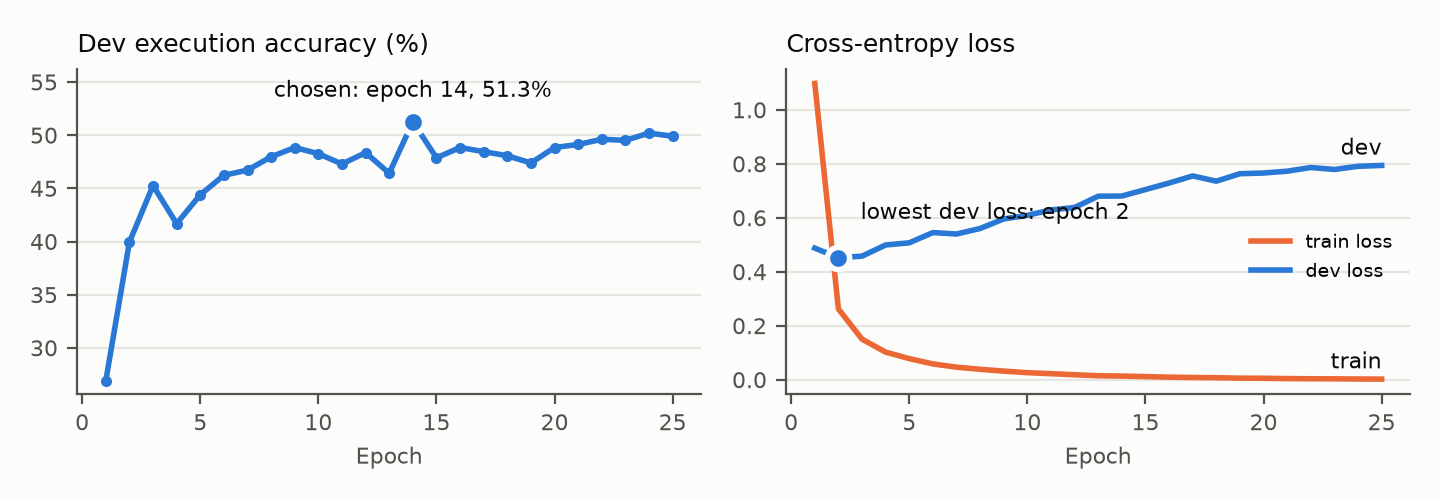
\includegraphics[width=0.8\linewidth,height=\textheight,keepaspectratio,alt={T5-base training (HPC job 398846). Left: greedy dev execution accuracy per epoch. Right: training and dev cross-entropy loss.}]{t5_training_curve.png}
\caption{T5-base training (HPC job 398846). Left: greedy dev execution
accuracy per epoch. Right: training and dev cross-entropy loss.}
\end{figure}

\subsection{Error analysis}\label{error-analysis}

\textbf{Outcome by difficulty (Spider test, T5-base).} Every question
ends in one of three outcomes: correct, ran but returned the wrong
answer, or invalid (did not run).

{\def\LTcaptype{none} % do not increment counter
\begin{longtable}[]{@{}
  >{\raggedright\arraybackslash}p{(\linewidth - 6\tabcolsep) * \real{0.2000}}
  >{\raggedleft\arraybackslash}p{(\linewidth - 6\tabcolsep) * \real{0.2667}}
  >{\raggedleft\arraybackslash}p{(\linewidth - 6\tabcolsep) * \real{0.2667}}
  >{\raggedleft\arraybackslash}p{(\linewidth - 6\tabcolsep) * \real{0.2667}}@{}}
\toprule\noalign{}
\begin{minipage}[b]{\linewidth}\raggedright
Difficulty
\end{minipage} & \begin{minipage}[b]{\linewidth}\raggedleft
Questions
\end{minipage} & \begin{minipage}[b]{\linewidth}\raggedleft
Beam: correct / wrong / invalid
\end{minipage} & \begin{minipage}[b]{\linewidth}\raggedleft
A + B: correct / wrong / invalid
\end{minipage} \\
\midrule\noalign{}
\endhead
\bottomrule\noalign{}
\endlastfoot
Easy & 470 & 373 / 47 / 50 & 393 / 64 / 13 \\
Medium & 857 & 470 / 138 / 249 & 565 / 189 / 103 \\
Hard & 463 & 188 / 92 / 183 & 227 / 129 / 107 \\
Extra hard & 357 & 116 / 61 / 180 & 155 / 97 / 105 \\
\textbf{All} & \textbf{2,147} & \textbf{1,147 / 338 / 662} &
\textbf{1,340 / 479 / 328} \\
\end{longtable}
}

A + B halves the invalid queries (662 → 328). Of the 334 queries it
rescues, 193 become correct and 141 run but give the wrong answer, so
the remaining errors shift from ``does not run'' to ``wrong meaning''.

{\def\LTcaptype{none} % do not increment counter
\begin{longtable}[]{@{}
  >{\raggedright\arraybackslash}p{(\linewidth - 6\tabcolsep) * \real{0.5479}}
  >{\raggedleft\arraybackslash}p{(\linewidth - 6\tabcolsep) * \real{0.1507}}
  >{\raggedleft\arraybackslash}p{(\linewidth - 6\tabcolsep) * \real{0.1507}}
  >{\raggedleft\arraybackslash}p{(\linewidth - 6\tabcolsep) * \real{0.1507}}@{}}
\toprule\noalign{}
\begin{minipage}[b]{\linewidth}\raggedright
Failure type (dev, out of 1,034)
\end{minipage} & \begin{minipage}[b]{\linewidth}\raggedleft
T5 beam
\end{minipage} & \begin{minipage}[b]{\linewidth}\raggedleft
T5 + A + B
\end{minipage} & \begin{minipage}[b]{\linewidth}\raggedleft
gpt-oss 0-shot
\end{minipage} \\
\midrule\noalign{}
\endhead
\bottomrule\noalign{}
\endlastfoot
Query does not run & 317 & 135 & 8 \\
\ldots{} ``no such column'' & 275 & 123 & 3 \\
\ldots{} ``no such table'' & 21 & 7 & 0 \\
Runs, but wrong tables & 44 & 80 & 69 \\
Runs, but wrong columns & 68 & 98 & 114 \\
Runs, but wrong clause structure & 20 & 31 & 68 \\
Runs, but wrong values & 12 & 11 & 67 \\
\end{longtable}
}

\textbf{Recurring patterns.}

\begin{itemize}
\tightlist
\item
  \textbf{Schema linking dominates T5's errors.} Most invalid queries
  reference columns that exist in a \emph{different} table,
  e.g.~\texttt{ORDER\ BY\ age} in \texttt{pets} when \texttt{age} is a
  student column and the pet column is \texttt{pet\_age}. A + B removes
  55\% of them.
\item
  \textbf{Valid but wrong.} A + B turns many crashing queries into ones
  that run, but some of those now use the wrong table or column.
  Execution checks cannot detect a query that runs but answers a
  different question; this is the method's main limit.
\item
  \textbf{Long schemas.} 24\% of training inputs exceed T5's 512-token
  limit and lose their last tables, so the model learns less about large
  databases.
\item
  \textbf{gpt-oss fails on meaning, not syntax.} Its errors are wrong
  values, extra columns and different conventions. Its EM (20.1\%) is
  far below its EX (78.6\%) because it writes correct SQL in its own
  style, e.g.~\texttt{COUNT(*)\ AS\ total\_singers},
  \texttt{LEFT\ JOIN}, explicit table aliases, which exact match counts
  as wrong.
\end{itemize}

\textbf{Qualitative examples.}

\begin{enumerate}
\def\labelenumi{\arabic{enumi}.}
\tightlist
\item
  \emph{``How much does the youngest dog weigh?''} (pets\_1). Beam:
  \texttt{ORDER\ BY\ age} (no such column in \texttt{pets}). A + B:
  \texttt{ORDER\ BY\ pet\_age}, correct.
\item
  \emph{``Which of the countries has the most car makers?''} (car\_1).
  Beam reads \texttt{CountryName} from \texttt{car\_makers}, where it
  does not exist. A + B joins \texttt{countries} and is correct.
\item
  \emph{``Show the stadium name and the number of concerts in each
  stadium.''} gpt-oss writes a \texttt{LEFT\ JOIN}, which also lists
  stadiums with zero concerts. It is a reasonable reading of the
  question, but differs from the gold answer, which uses an inner join;
  the benchmark's conventions affect the score.
\item
  \emph{A coincidental match.} For ``the student who has a cat that is
  age 3'' (pets\_1), A + B's query drops the ``cat'' condition but still
  returns the right student, because the only 3-year-old pet in the
  database is a cat. EX counts it correct; EM does not.
\end{enumerate}

\textbf{Mitigation.} Ranking schema items before decoding (as RESDSQL
does) would shorten long inputs and give the model fewer wrong names to
choose from; checking a query's meaning, for example by asking a second
model whether the result answers the question, could catch
valid-but-wrong queries.

\subsection{Challenges}\label{challenges}

{\def\LTcaptype{none} % do not increment counter
\begin{longtable}[]{@{}
  >{\raggedright\arraybackslash}p{(\linewidth - 4\tabcolsep) * \real{0.3333}}
  >{\raggedright\arraybackslash}p{(\linewidth - 4\tabcolsep) * \real{0.3333}}
  >{\raggedright\arraybackslash}p{(\linewidth - 4\tabcolsep) * \real{0.3333}}@{}}
\toprule\noalign{}
\begin{minipage}[b]{\linewidth}\raggedright
Stage
\end{minipage} & \begin{minipage}[b]{\linewidth}\raggedright
Challenge
\end{minipage} & \begin{minipage}[b]{\linewidth}\raggedright
How we solved it
\end{minipage} \\
\midrule\noalign{}
\endhead
\bottomrule\noalign{}
\endlastfoot
Tokenisation & T5's vocabulary has no \texttt{\textless{}}, so 320
training queries could never be generated correctly & Added
\texttt{\textless{}} and \texttt{\textless{}=} as new tokens before
fine-tuning \\
Model selection & Dev \emph{loss} was best at epoch 2, but that model
still wrote broken SQL (41\% EX) & Selected the checkpoint by dev
\emph{execution accuracy} after every epoch (epoch 14, 51\%) \\
Long inputs & 24\% of training schemas exceed 512 tokens & Kept
truncation; noted as a limitation (schema ranking is the fix) \\
LLM on the HPC & gpt-oss's 4-bit kernels need C headers missing on the
cluster & Loaded the model in 16-bit precision (about 42 GB) \\
Shared GPUs & Few-shot prompts ran out of memory when other users shared
the card & Smaller batches, a memory-allocator setting, and splitting
the run into halves \\
Cluster limits & One GPU job per user and a 2-hour time limit & One job
per setting; checkpoint saved after every improving epoch \\
Live demo & The HPC queue can delay live training during the viva & Demo
trains t5-small on the laptop (about 3 minutes), with the HPC run as an
option \\
Fair evaluation & Dev chose the checkpoint and settings, so dev scores
are optimistic & Final claims use the test set, run once \\
\end{longtable}
}

\section{Conclusion}\label{conclusion}

On one benchmark with one evaluator, accuracy rises from under 10\% with
rules and LSTMs, to 54\% by fine-tuning a pre-trained T5-base, and to
79\% with a 20-billion-parameter LLM used without any training. This
tracks the field's shift from hand-written rules, to models trained from
scratch, to pre-trained models adapted with little or no task data.

Our contribution, schema-constrained beam search plus execution-guided
reranking, adds 9.0 points to T5-base on the held-out Spider test set
(10.3 on dev) without retraining by fixing its dominant error:
references to tables and columns that do not exist. It is simple, works
with any seq2seq model and any SQLite database, and helps most on join
queries. It cannot fix queries that run but answer the wrong question,
and it adds little to an LLM that rarely writes invalid SQL. Exact match
proved unsuitable for judging LLM output, so execution accuracy should
be the primary metric. Natural next steps are schema ranking before
decoding and checking whether a query's result actually answers the
question.

\section*{References}\label{references}
\addcontentsline{toc}{section}{References}

\footnotesize

\begin{itemize}
\tightlist
\item
  Bahdanau, D., Cho, K., Bengio, Y. (2015). Neural machine translation
  by jointly learning to align and translate. \emph{ICLR}.
\item
  Chen, X., Lin, M., Schärli, N., Zhou, D. (2024). Teaching large
  language models to self-debug. \emph{ICLR}.
\item
  Gao, D., Wang, H., Li, Y., et al.~(2024). Text-to-SQL empowered by
  large language models: a benchmark evaluation. \emph{VLDB}.
\item
  Hochreiter, S., Schmidhuber, J. (1997). Long short-term memory.
  \emph{Neural Computation}.
\item
  Li, H., Zhang, J., Li, C., Chen, H. (2023). RESDSQL: decoupling schema
  linking and skeleton parsing for Text-to-SQL. \emph{AAAI}.
\item
  McNemar, Q. (1947). Note on the sampling error of the difference
  between correlated proportions or percentages. \emph{Psychometrika}.
\item
  OpenAI (2025). gpt-oss-120b and gpt-oss-20b model card.
\item
  Popescu, A.-M., Etzioni, O., Kautz, H. (2003). Towards a theory of
  natural language interfaces to databases. \emph{IUI}.
\item
  Pourreza, M., Rafiei, D. (2023). DIN-SQL: decomposed in-context
  learning of Text-to-SQL with self-correction. \emph{NeurIPS}.
\item
  Raffel, C., Shazeer, N., Roberts, A., et al.~(2020). Exploring the
  limits of transfer learning with a unified text-to-text transformer.
  \emph{JMLR}.
\item
  Scholak, T., Schucher, N., Bahdanau, D. (2021). PICARD: parsing
  incrementally for constrained auto-regressive decoding from language
  models. \emph{EMNLP}.
\item
  See, A., Liu, P. J., Manning, C. D. (2017). Get to the point:
  summarization with pointer-generator networks. \emph{ACL}.
\item
  Shaw, P., Chang, M.-W., Pasupat, P., Toutanova, K. (2021).
  Compositional generalization and natural language variation: can a
  semantic parsing approach handle both? \emph{ACL}.
\item
  Sutskever, I., Vinyals, O., Le, Q. V. (2014). Sequence to sequence
  learning with neural networks. \emph{NeurIPS}.
\item
  Vaswani, A., Shazeer, N., Parmar, N., et al.~(2017). Attention is all
  you need. \emph{NeurIPS}.
\item
  Vinyals, O., Fortunato, M., Jaitly, N. (2015). Pointer networks.
  \emph{NeurIPS}.
\item
  Wang, B., Shin, R., Liu, X., Polozov, O., Richardson, M. (2020).
  RAT-SQL: relation-aware schema encoding and linking for Text-to-SQL
  parsers. \emph{ACL}.
\item
  Wong, Y. W., Mooney, R. (2007). Learning synchronous grammars for
  semantic parsing with lambda calculus. \emph{ACL}.
\item
  Xu, X., Liu, C., Song, D. (2017). SQLNet: generating structured
  queries from natural language without reinforcement learning.
  \emph{arXiv:1711.04436}.
\item
  Yu, T., Zhang, R., Yang, K., et al.~(2018). Spider: a large-scale
  human-labeled dataset for complex and cross-domain semantic parsing
  and Text-to-SQL task. \emph{EMNLP}.
\item
  Zettlemoyer, L., Collins, M. (2005). Learning to map sentences to
  logical form. \emph{UAI}.
\item
  Zhong, R., Yu, T., Klein, D. (2020). Semantic evaluation for
  Text-to-SQL with distilled test suites. \emph{EMNLP}.
\item
  Zhong, V., Xiong, C., Socher, R. (2017). Seq2SQL: generating
  structured queries from natural language using reinforcement learning.
  \emph{arXiv:1709.00103}.
\end{itemize}

\end{document}
